\documentclass{article}
\usepackage[fleqn]{amsmath}
\usepackage[pdftex]{graphicx}
\usepackage{url}


\begin{document}

\title{Seamless multiprojector display}
\author{Pranav Kant Gaur}

\maketitle

\begin{abstract}
This document describes the development of a multiprojector display system. It also describes the novel \textit{cross ratio} based approach for recovering the projection region lost due to non-zero feature size. It thereby overcomes the limitations of method introduced by Brown's\cite{1} approach for multiprojector geometric alignment. Possibility of utilization of full projection region also allows for completely arbitrary arrangement of projectors eliminating the requirement for neighbor projectors to overlap atleast upto their outermost feature boundaries. This approach completely removes required manual intervention involved in interactive alignment based multiprojector display systems(like Compiz plugin based alignment). Developed system has rear projection configuration, which adds additional problem of \textit{view-dependent} bright \textit{Hot spot} formation on projection screen. This problem is still under investigation.
\end{abstract}

\section{Problem definition}
Given perspectively distorted projections of a MXN grid of projectors on a planar surface, we need to find mapping between between original projector buffer image and warped image. Warped image is such that when projected in combination with that of other projectors results in a geometrically continous and rectangular display with intensity seamlessness at the junction between adjacent projectors. This problem is referred in literature as \textbf{\textit{Multiprojector geometric alignment and edge blending}}.

\section{System setup}
System is composed of:
\begin{enumerate}
\item Projector array
\item Master and slave workstation arrangement
\item PC running geometric alignment and edge blendng software
\item Camera
\item Projection screen
\end{enumerate}
    It is a rear projection system. Grid of projectors project image onto a common screen. Final target is to provide a geometrically and radiometrically seamless high resolution display on screen. Informally, the displayed scene should appear as if projected through a single wide field of view projector. Figure \ref{setup} shows our display screen with workstation cluster and a camera which is used as a visual feedback device. Figure \ref{projs} shows the 3X3 projector grid in our rear projection display system.
\begin{figure}[ht]
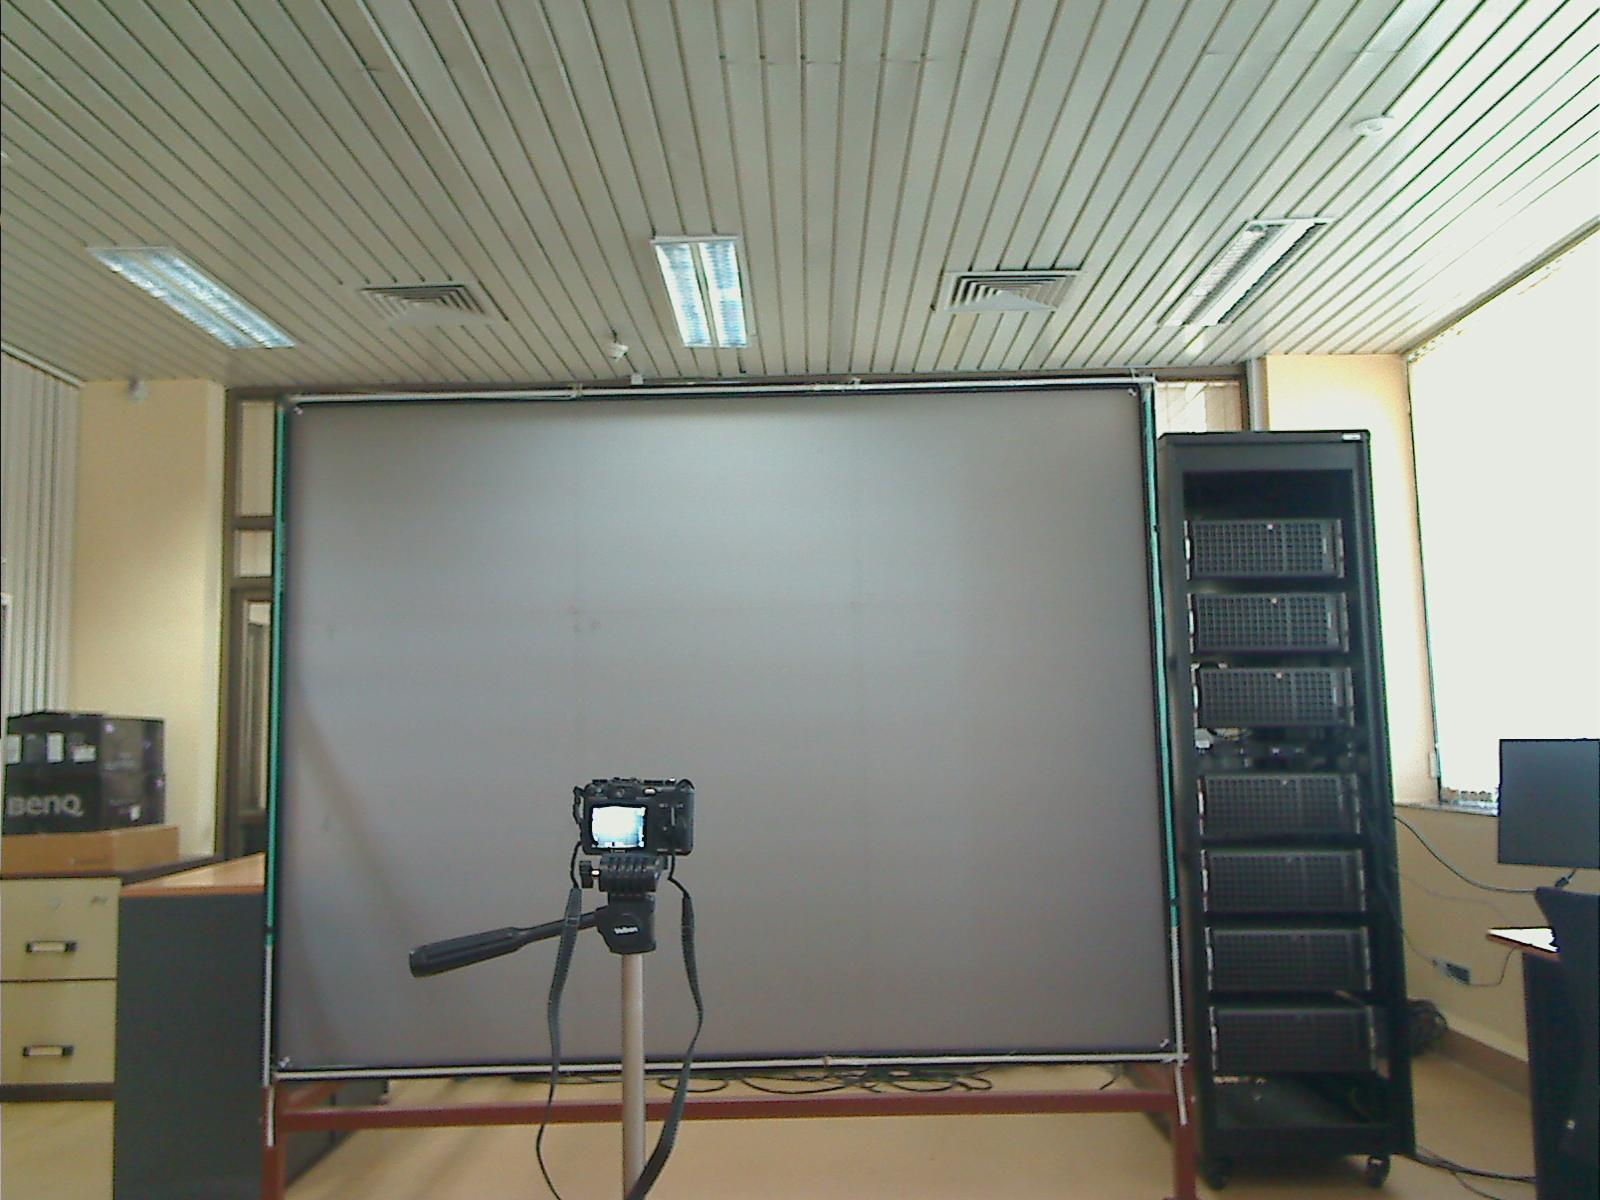
\includegraphics[width=11cm,height=8cm]{figures/setup.jpg}
\caption{System setup}
\label{setup}
\end{figure}

\begin{figure}
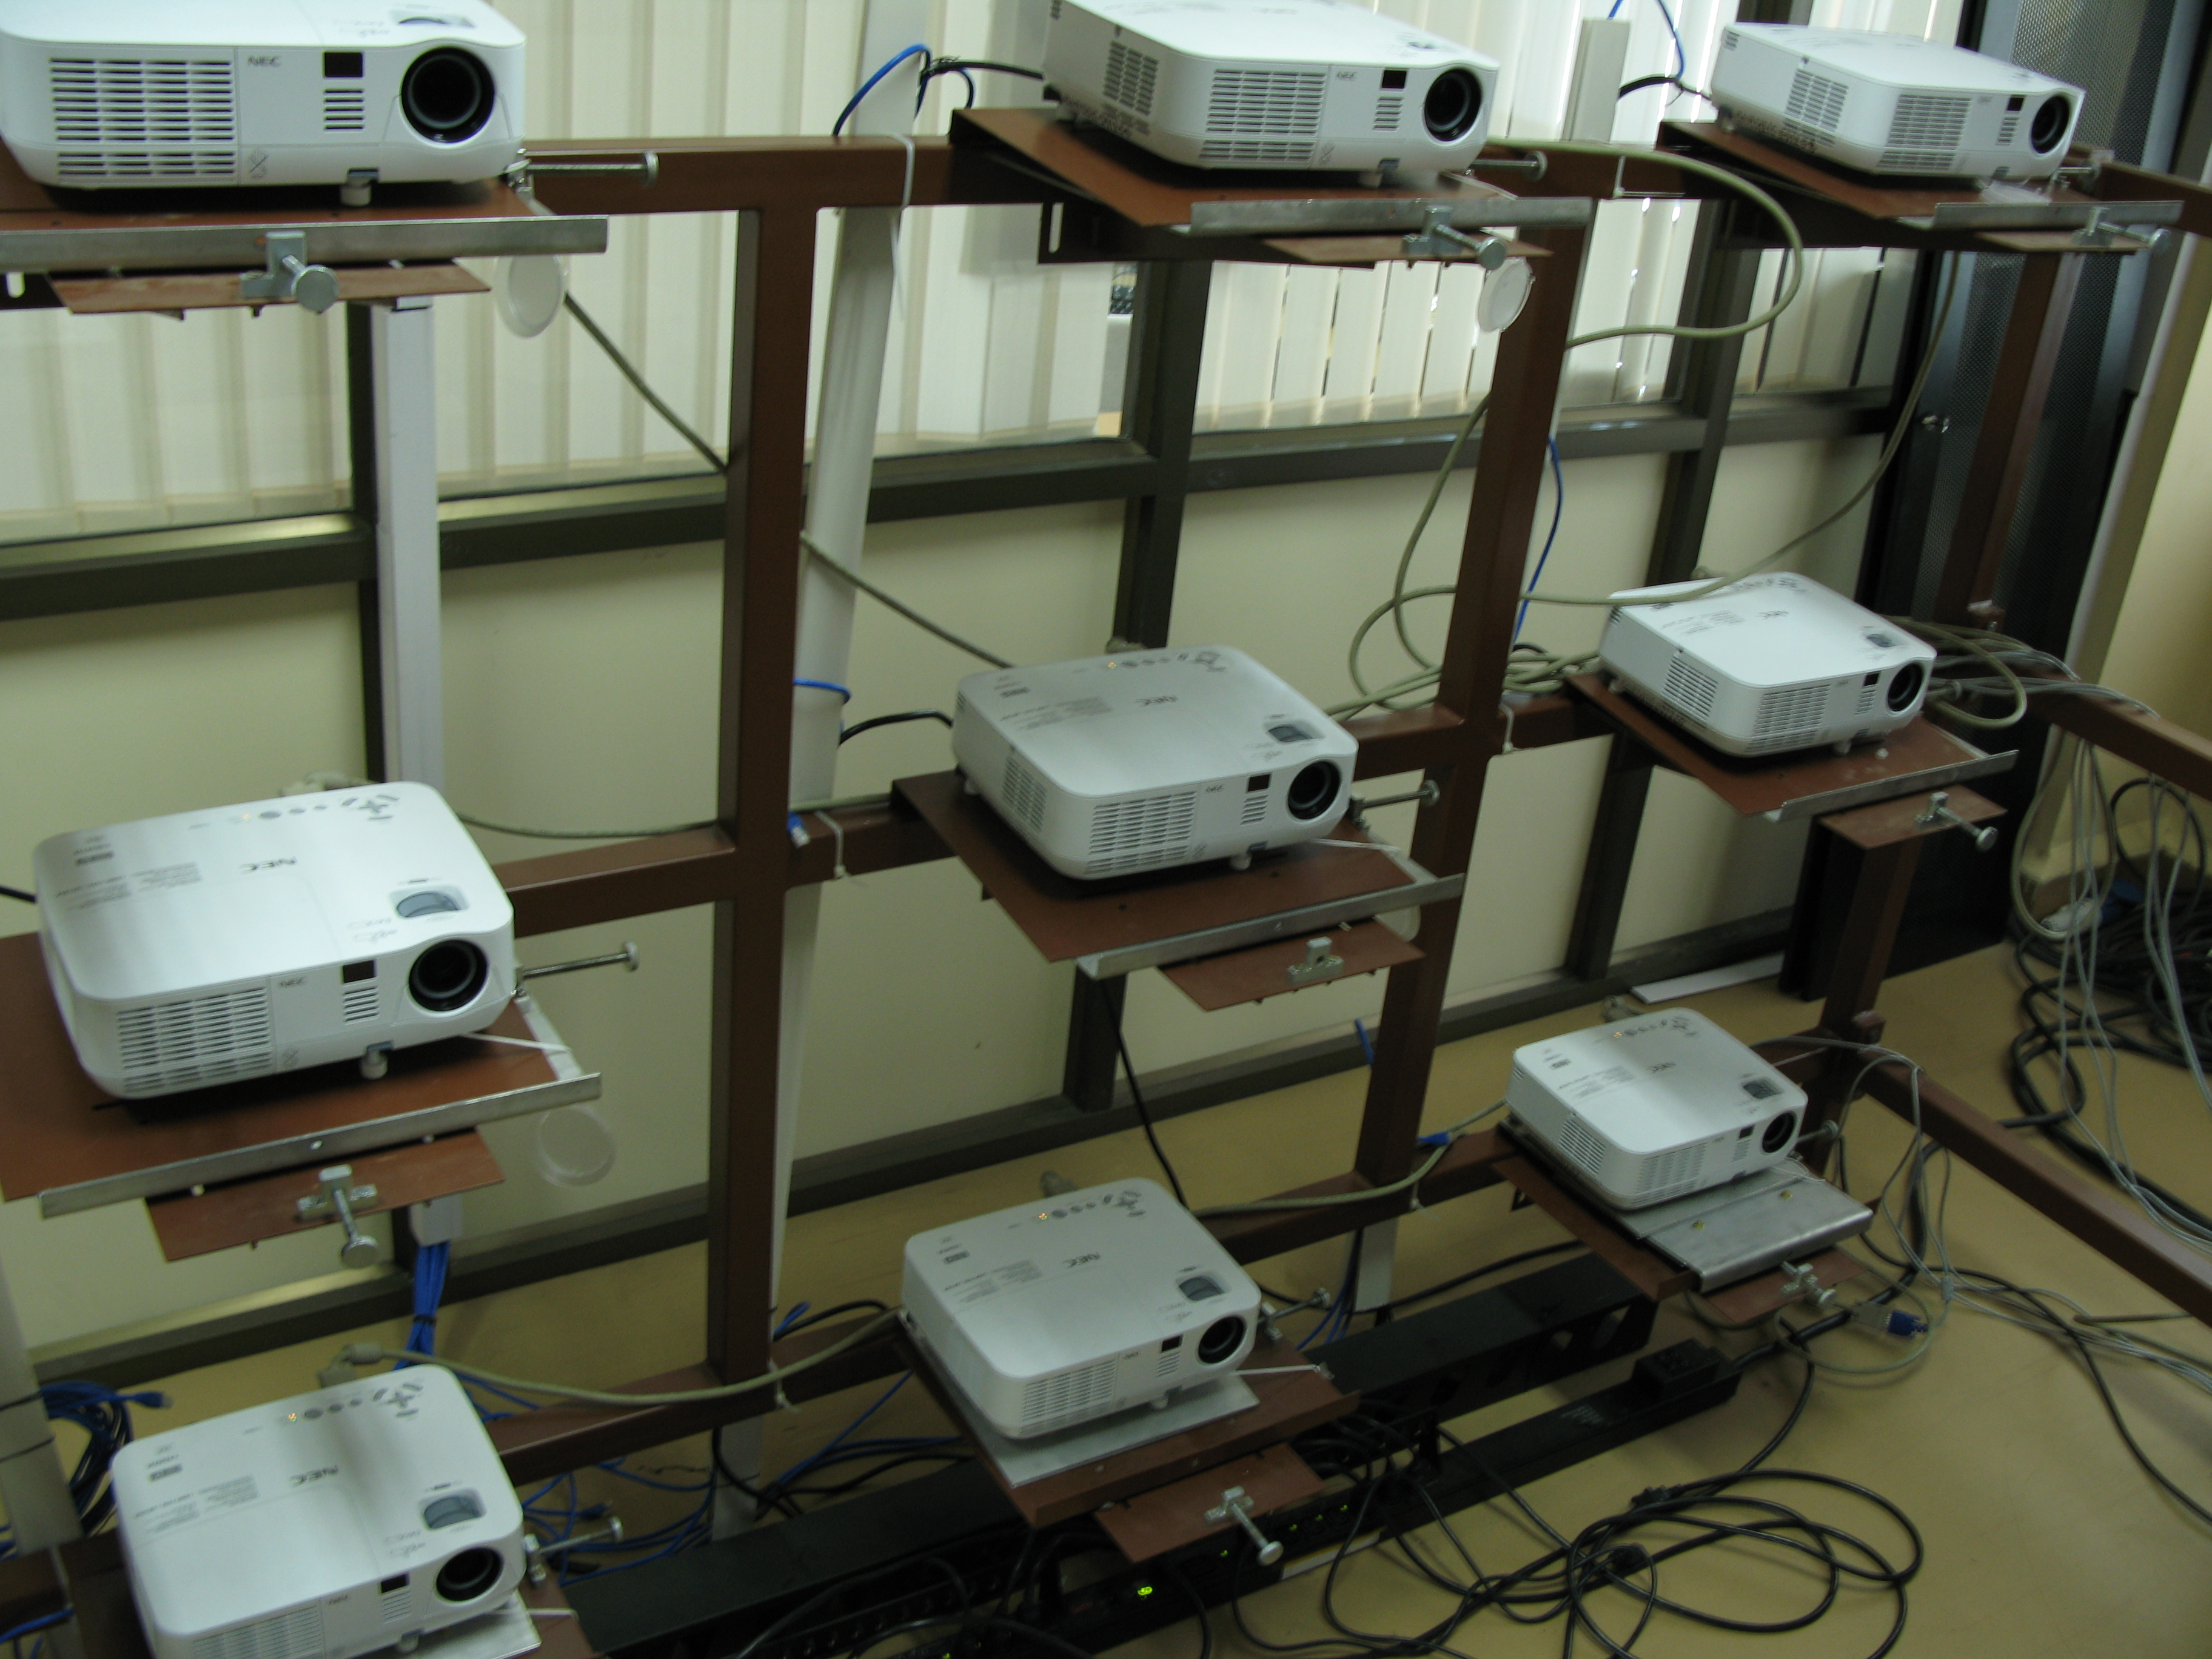
\includegraphics[width=11cm,height=8cm]{figures/projs.jpg}
\caption{3X3 rear projection grid}
\label{projs}
\end{figure}

\section{Solutions proposed in literature}
In our work, we have considered approaches which utilize camera as a feedback device to compute warping information. Earlier attempted approach was based on the concept of \textit{Homography}\cite{5}. It establishes planar projective mapping between screen and camera followed by that between camera and projector. Utilizing combination of these homographies it computes relation between screen and projector. Since it is assumed that position of final projection on screen is known, corresponding projector space coordinates can be easily computed utilizing screen to projector homography. This gives the warping information. \newline
Homography between screen-camera, $H_{sc}$
\begin{equation}
x_{c}=H_{sc}*x_{s}
\end{equation}
Similarly, homography between camera-projector, $H_{cp}$
\begin{equation}
x_{p}=H_{cp}*x_{c}
\end{equation}

Therefore, using screen-projector homography, $H_{sp}$ gives,
\begin{equation}
x_{p}=\underbrace{H_{sc}*H_{cp}}_{H_{sp}}*x_{s}
\end{equation}



Brown's[1] approach relaxes that assumption and instead allows for a casual positioning of projectors. It aims to create geometrically seamless and rectangular image in camera space which guarantees geometrical seamlessness on the screen. But it does not guarantee rectangular output on the screen. 


\subsection{Demerits of the above approaches}
\begin{enumerate}
\item Earlier approach:
\begin{enumerate}
\item Assumes accurate positioning of features on the screen.
\item Assumption of planarity of the screen. But in practice screens may not be perfectly planar.
\item Pre-positioning of projection region results in relatively stringent physical constraints on placement of projectors.
\end{enumerate}
\item Brown's\cite{1} approach:
\begin{enumerate}
\item Usable projection region is limited by size of features used for geometric registration.
\item Rectangular output is ensured in camera but not on the display screen. 
\end{enumerate}
\end{enumerate}
However, Brown's approach has advantage of being much more flexible in terms of projector placement, hence this was chosen as our base approach on top of which we have removed the limitations (a) and (b) mentioned here.


\section{Solution proposed in this work}
    We have proposed using projective invariant called \textbf{\textit{cross-ratio}} to recover the projection region lost due to non-zero feature size. In addition, we have used screen-to-camera homography to ensure rectangular output on the screen. However, this also introduces assumptions in basic Brown's approach. Cross-ratio being planer projective invariant demands that screen must be planar. Further, accurate computation of screen to camera homography requires accurate positioning of screen points.

\subsubsection{Cross-ratio invariance}
  Cross ratio is a planer projective invariant. It states that: Given 4 collinear points A,B,C,D, their cross-ratio $CR$:
\begin{equation} 
CR[A,B,C,D]=(AC/AD)/(BC/BD)
\end{equation}
will be preserved under perspective projection. Therefore, assuming planer perspective projection of features from projector to screen and from screen to camera, we can recover coordinates of an unknown point(say 'A') in camera space given coordinates of other three(i.e.,'B','C','D' are known). \newline \newline
Let $A_p$,$B_p$,$C_p$,$D_p$ be the coordinates of 4 collinear points in projector space and $A_c$,$B_c$,$C_c$,$D_c$ be the corresponding projection in camera space. Here, $B_c$,$C_c$ and $D_c$ are known whereas $A_c$ is unknown but $A_p$,$B_p$,$C_p$,$D_p$ are all known. Let us further represent the line joining $A_c$,$B_c$,$C_c$,$D_c$ in parametric form as:
\begin{equation}
\begin{aligned}
x_t=B_c^x+t*(D_c^x-B_c^x)\\
y_t=B_c^y+t*(D_c^y-B_c^y)
\end{aligned}
\label{paramet}
\end{equation}
where, $(x_t,y_t)$ are parametric coordinates of an unknown point(in our case $A_c$)\newline
Utilizing cross ratio invariance yields following relation:
\begin{equation}
CR_p=\frac{AC_c*BD_c}{BC_c*AD_c}
\end{equation}
Here $CR_p$ is the cross ratio computed in projector-space. Using equation 5, we get quadratic equation with following possible solutions:
\begin{equation}
\begin{aligned}
t_1=\frac{-b+\sqrt{b^{2}-4ac}}{2a}\\
t_2=\frac{-b-\sqrt{b^{2}-4ac}}{2a}
\end{aligned}
\end{equation}
where,\newline
Let,\newline
$delta={CR_p*(\frac{BC_c}{BD_c})}^2$\newline
Then,\newline
$a=(1-delta)*BD_c^2$\newline
$b=2*{(D_c^x-B_c^x)*(B_c^x-C_c^x)+(D_c^y-B_c^y)*(B_c^y-C_c^y)+BD_c^{2}*delta}$\newline
$c=BC_c^2-delta*BD_c^2$
\newline \newline
Based on the convention of the chosen coordinate system, only one of $t_1$ or $t_2$ will be the valid position of the unknown point $A_c$.

\section{Basic algoritms}
\begin{enumerate}
\item Geometric alignment:
\begin{enumerate}    
\item Feature detection:
\begin{enumerate}
\item Projector projects checkerboard features.
\item Camera captures features.
\item Since collinearity is invariant under projective transformation, features collinear in projector image must also be 		      collinear in camera space. To account for this detected locations of features in camera image is regularized by explicitly enforcing collinearity constraint. Specifically, each feature is computed as intersection of vertical and horizontal fitted lines.

\item Once the features are regularized, lost projection region at the boundary are recovered using Cross-ratio constraint(using equation 7).
\item Regularized positions of newly computed coordinates are computed by fitting line on collinear points and computing intersections.
\end{enumerate}
\item Warping map computation:
\begin{enumerate}	     
\item Local bounding boxes are computed for each projection region in camera space. These boxes are the convex hulls enclosing all features of a projector recovered in steps (i)-(v) in feature detection phase.

\item A global bounding box is computed which is convex hull enclosing all local bounding boxes.

\item This global bounding box acts like a global coordinate system containing all local bounding boxes and hence all the 		      detected features. A scale for both box width and height is computed which corresponds to the maximum width and height among that of all local bounding boxes.
 
\item These factors map position of individual local bounding boxes to positions of tiles in chromium configuration.

\item To compute texture coordinates corresponding to all features of a projector, normalized coordinates of all features are 	            computed with respect to its local bounding box origin.
\end{enumerate}
\end{enumerate}
These steps give Chromium tile configuration and Vertex-texture mapping for each projector.

\item Edge blending:
\begin{enumerate}
\item Transform detected coordinates to global frame in chromium coordinates system.
\item Compute polygons bounding the detected corners for each projector.
\item Scan chromium image space and for each pixel, check which projector(s) share it.
\item For every sharing projector, assign that pixel the id of that projector.
\item Compute alpha weight of each projector based on distance transform value at that pixel for each projector.
\end{enumerate}
These steps give alpha map for each projector which is a 2D array(with same dimensions as of projector image) with value corresponding to each pixel varying from 0 to 255. Alpha weight at any pixel represents its transparency.
\end{enumerate}




\section{Practical implementation}
In this section, implementation details are described which include software architecture of multiprojector display system and hardware used for our experiments.

\subsection{Software architecture}
Software system is composed of geometric alignment module and edge blending module. Geometric alignment module computes vertex-texture map and chromium tile configuration for each projector. Edge blending module computes the alpha weights for each projector based on region of overlap among neighboring projectors. These information are sent to Master machine which runs chromium service to appropriately distribute alpha maps and vertex-texture mapping to individual machines driving projectors.



\subsection{Hardware configuration}
Hardware used for testing our approach includes:
\begin{enumerate}
\item PC: Intel Core i3 CPU 550 @ 3.20GHz running Ubuntu 12.04(64-bit)
\item Cluster: Each workstation with 2 x Intel Xeon Six Core Processor X5670 with NVIDIA Quadro FX 4600 cards 
\item Network(PC-cluster): Connected through local ethernet network
\item Network(Cluster-projector): Connected through VGA cables
\item Screen: Acryllic glass sheet with gain 1.6 from ScreenTech(Model: ST-Pro-DC)		
\item Camera: Canon PowerShot G7 at 3648X2736 resolution
\item Projector(s): NEC V300X at 1024X768 resolution
\end{enumerate}

\subsection{Hardware setup}
Projectors are connected through slave machines\{workstations\}. Single slave drives 3 projectors\{a row of display grid in our case\}. So, there are 3 slave workstations for 3X3 grid of projectors. Each slave runs chromium service to receive and accordingly texture map images to be projected by individual projectors under its control. Warping map, chromium tile configuration and blend map are generated on remote machine connected to the cluster\{master+slave arrangement\} through local network connection over Ethernet.



\section{Software dependencies}
OpenCV version 2.4 is used for camera image processing specifically, corner detection, image undistortion and camera calibration. GPhoto2(version 2.5.2) library is used for interfacing digital camera. Chromium(version 1.9)\cite{4} was modified to provide geometric correction and edge blending capability. Indigenously developed Control panel(version 2.0.32) software was used for logging into slave machines from master workstation.


   

\section{Results}
Figure \ref{non_cross_rat} shows the projection region without cross ratio and figure \ref{cross_rat} shows final output utilizing cross ratio constraint. Both renderings are on same physical configuration of projectors. Full projection region was utilized in cross ratio approach\{refer fig. \ref{cross_rat}\} whereas projection region in approach by Brown\cite{1} was limited by feature size as shown in figure \ref{non_cross_rat}. \newline 
Further, it can be inferred that in same physical configuration of projectors, the cross ratio based approach allows for more inter-projector overlap leading to more realistic alpha maps as can be compared in figures \ref{non_cross_rat} and \ref{cross_rat}. Consequently, boundaries are more visible in figure \ref{non_cross_rat} as compared to those in figure \ref{cross_rat}.

\begin{figure}
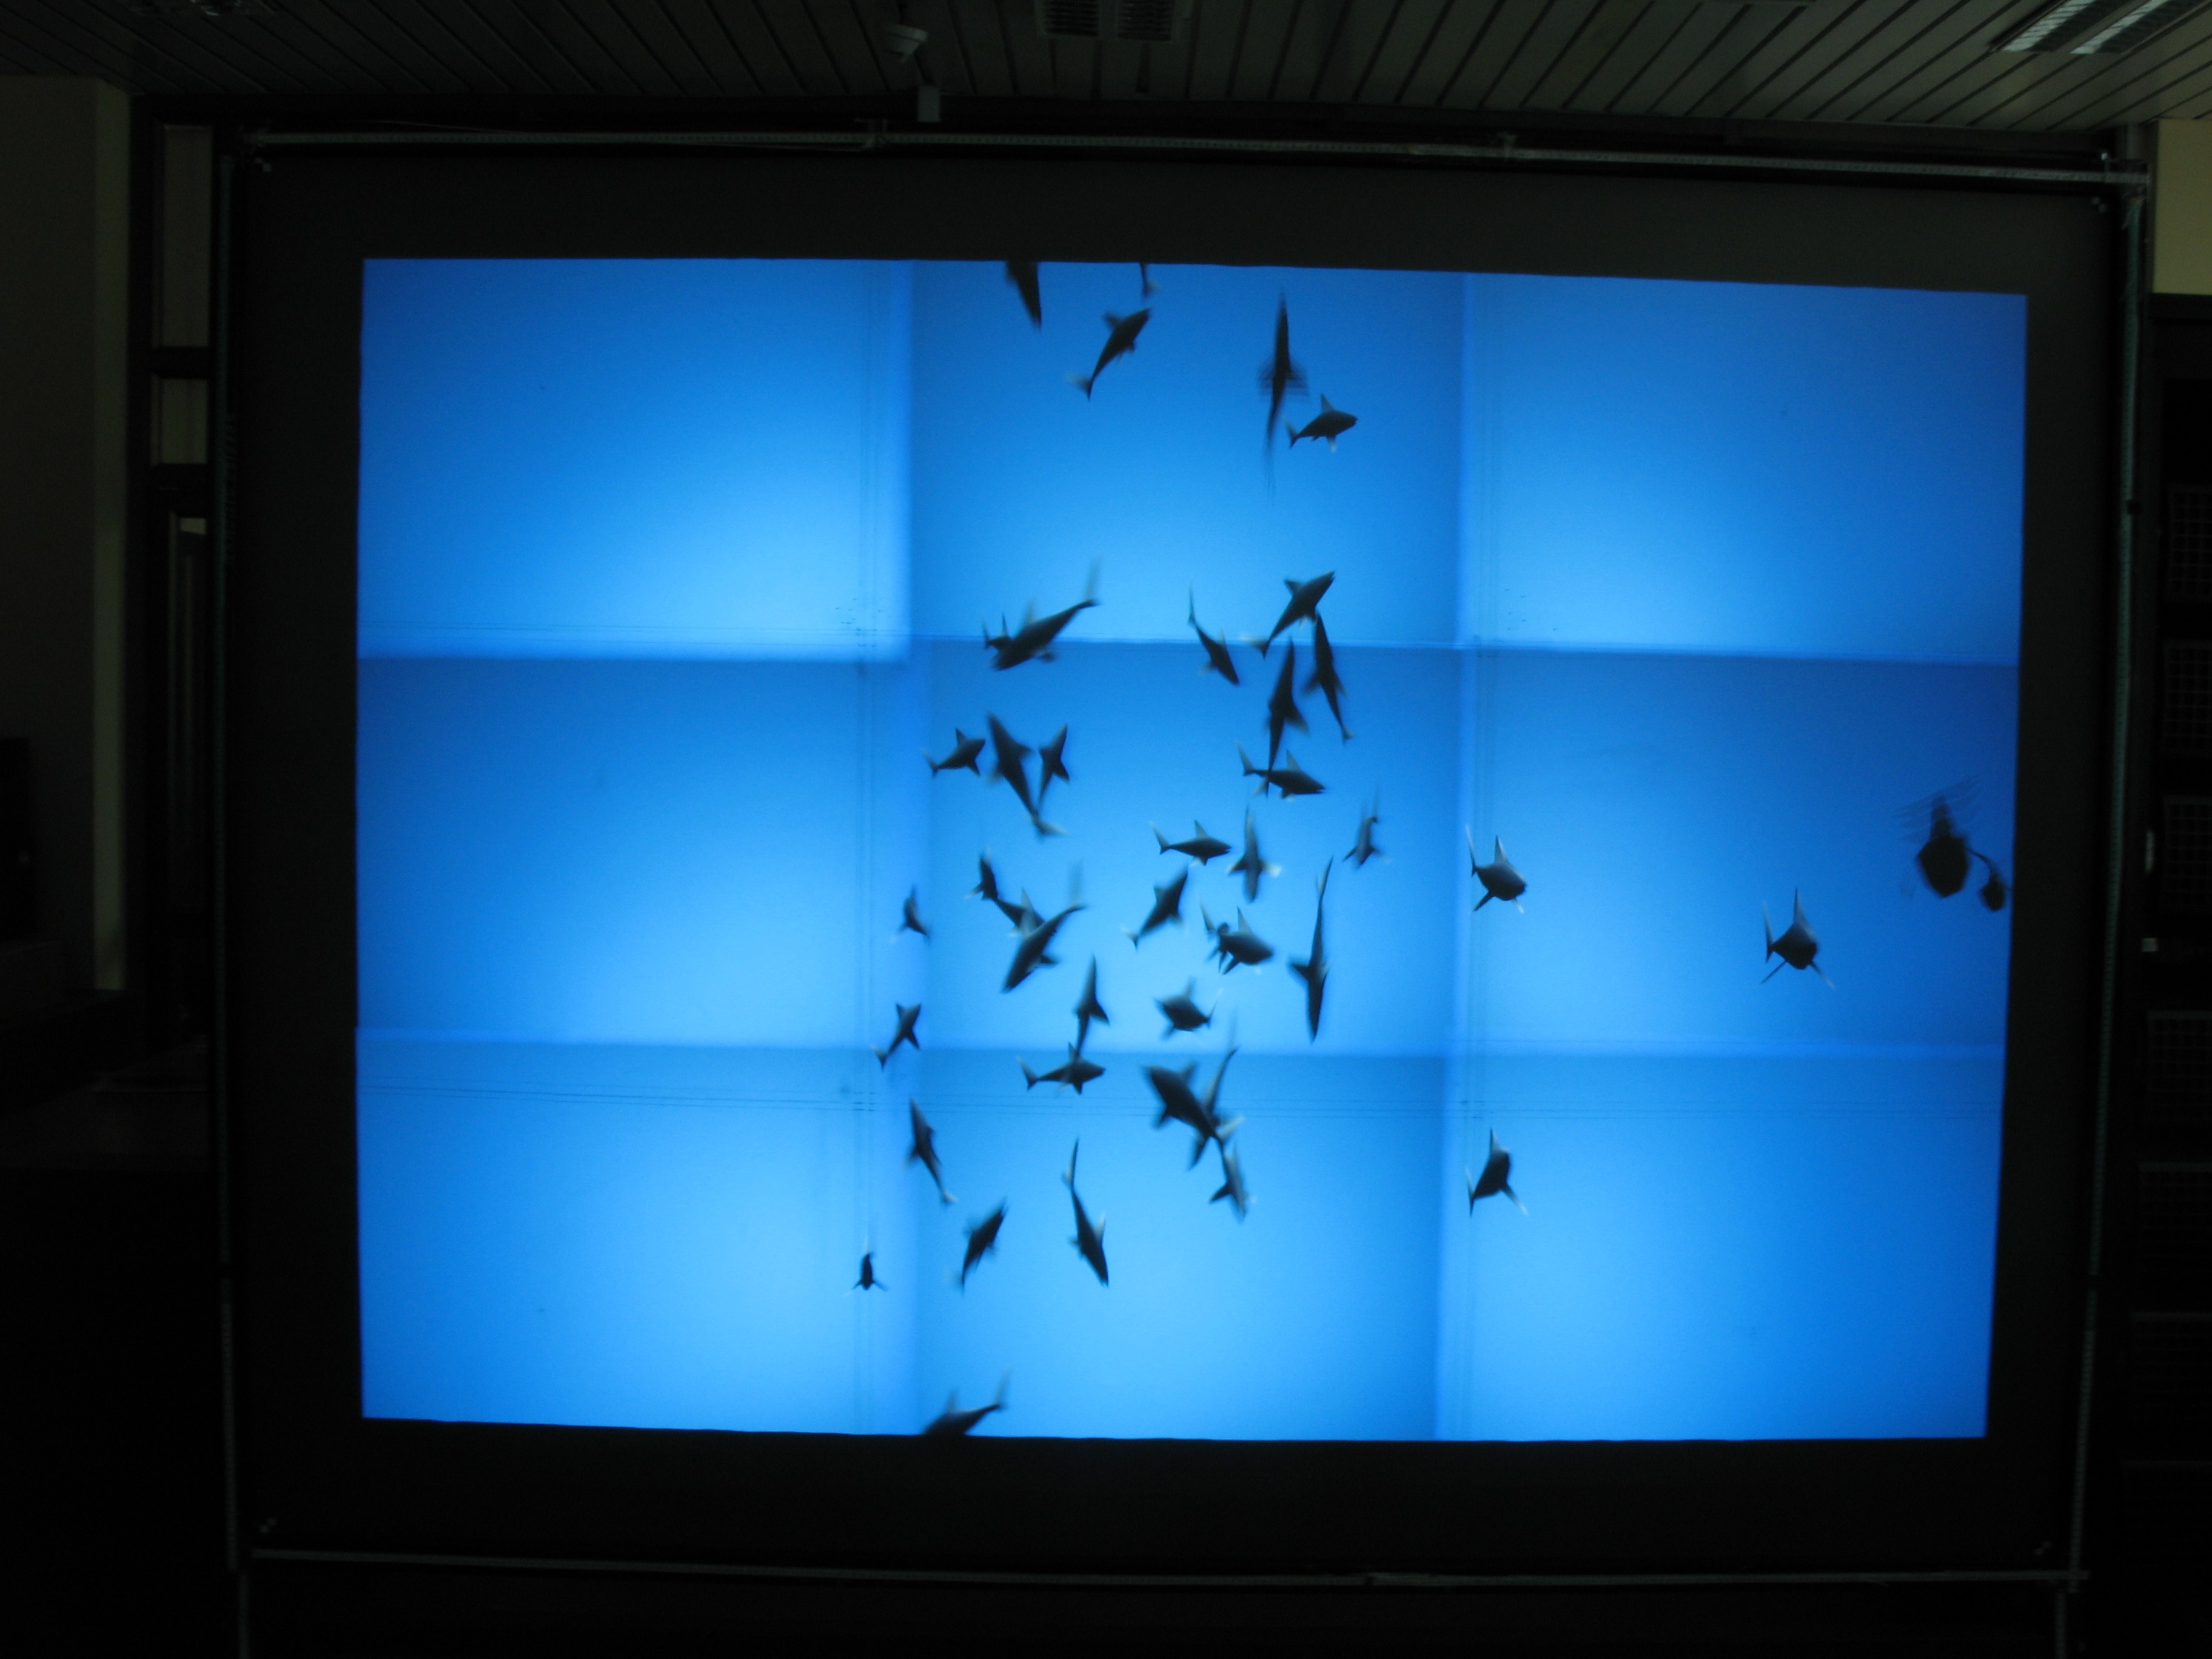
\includegraphics[width=11cm,height=8cm]{figures/without_cross_rat.jpg}
\caption{Without cross ratio}
\label{non_cross_rat}
\end{figure}


\begin{figure}
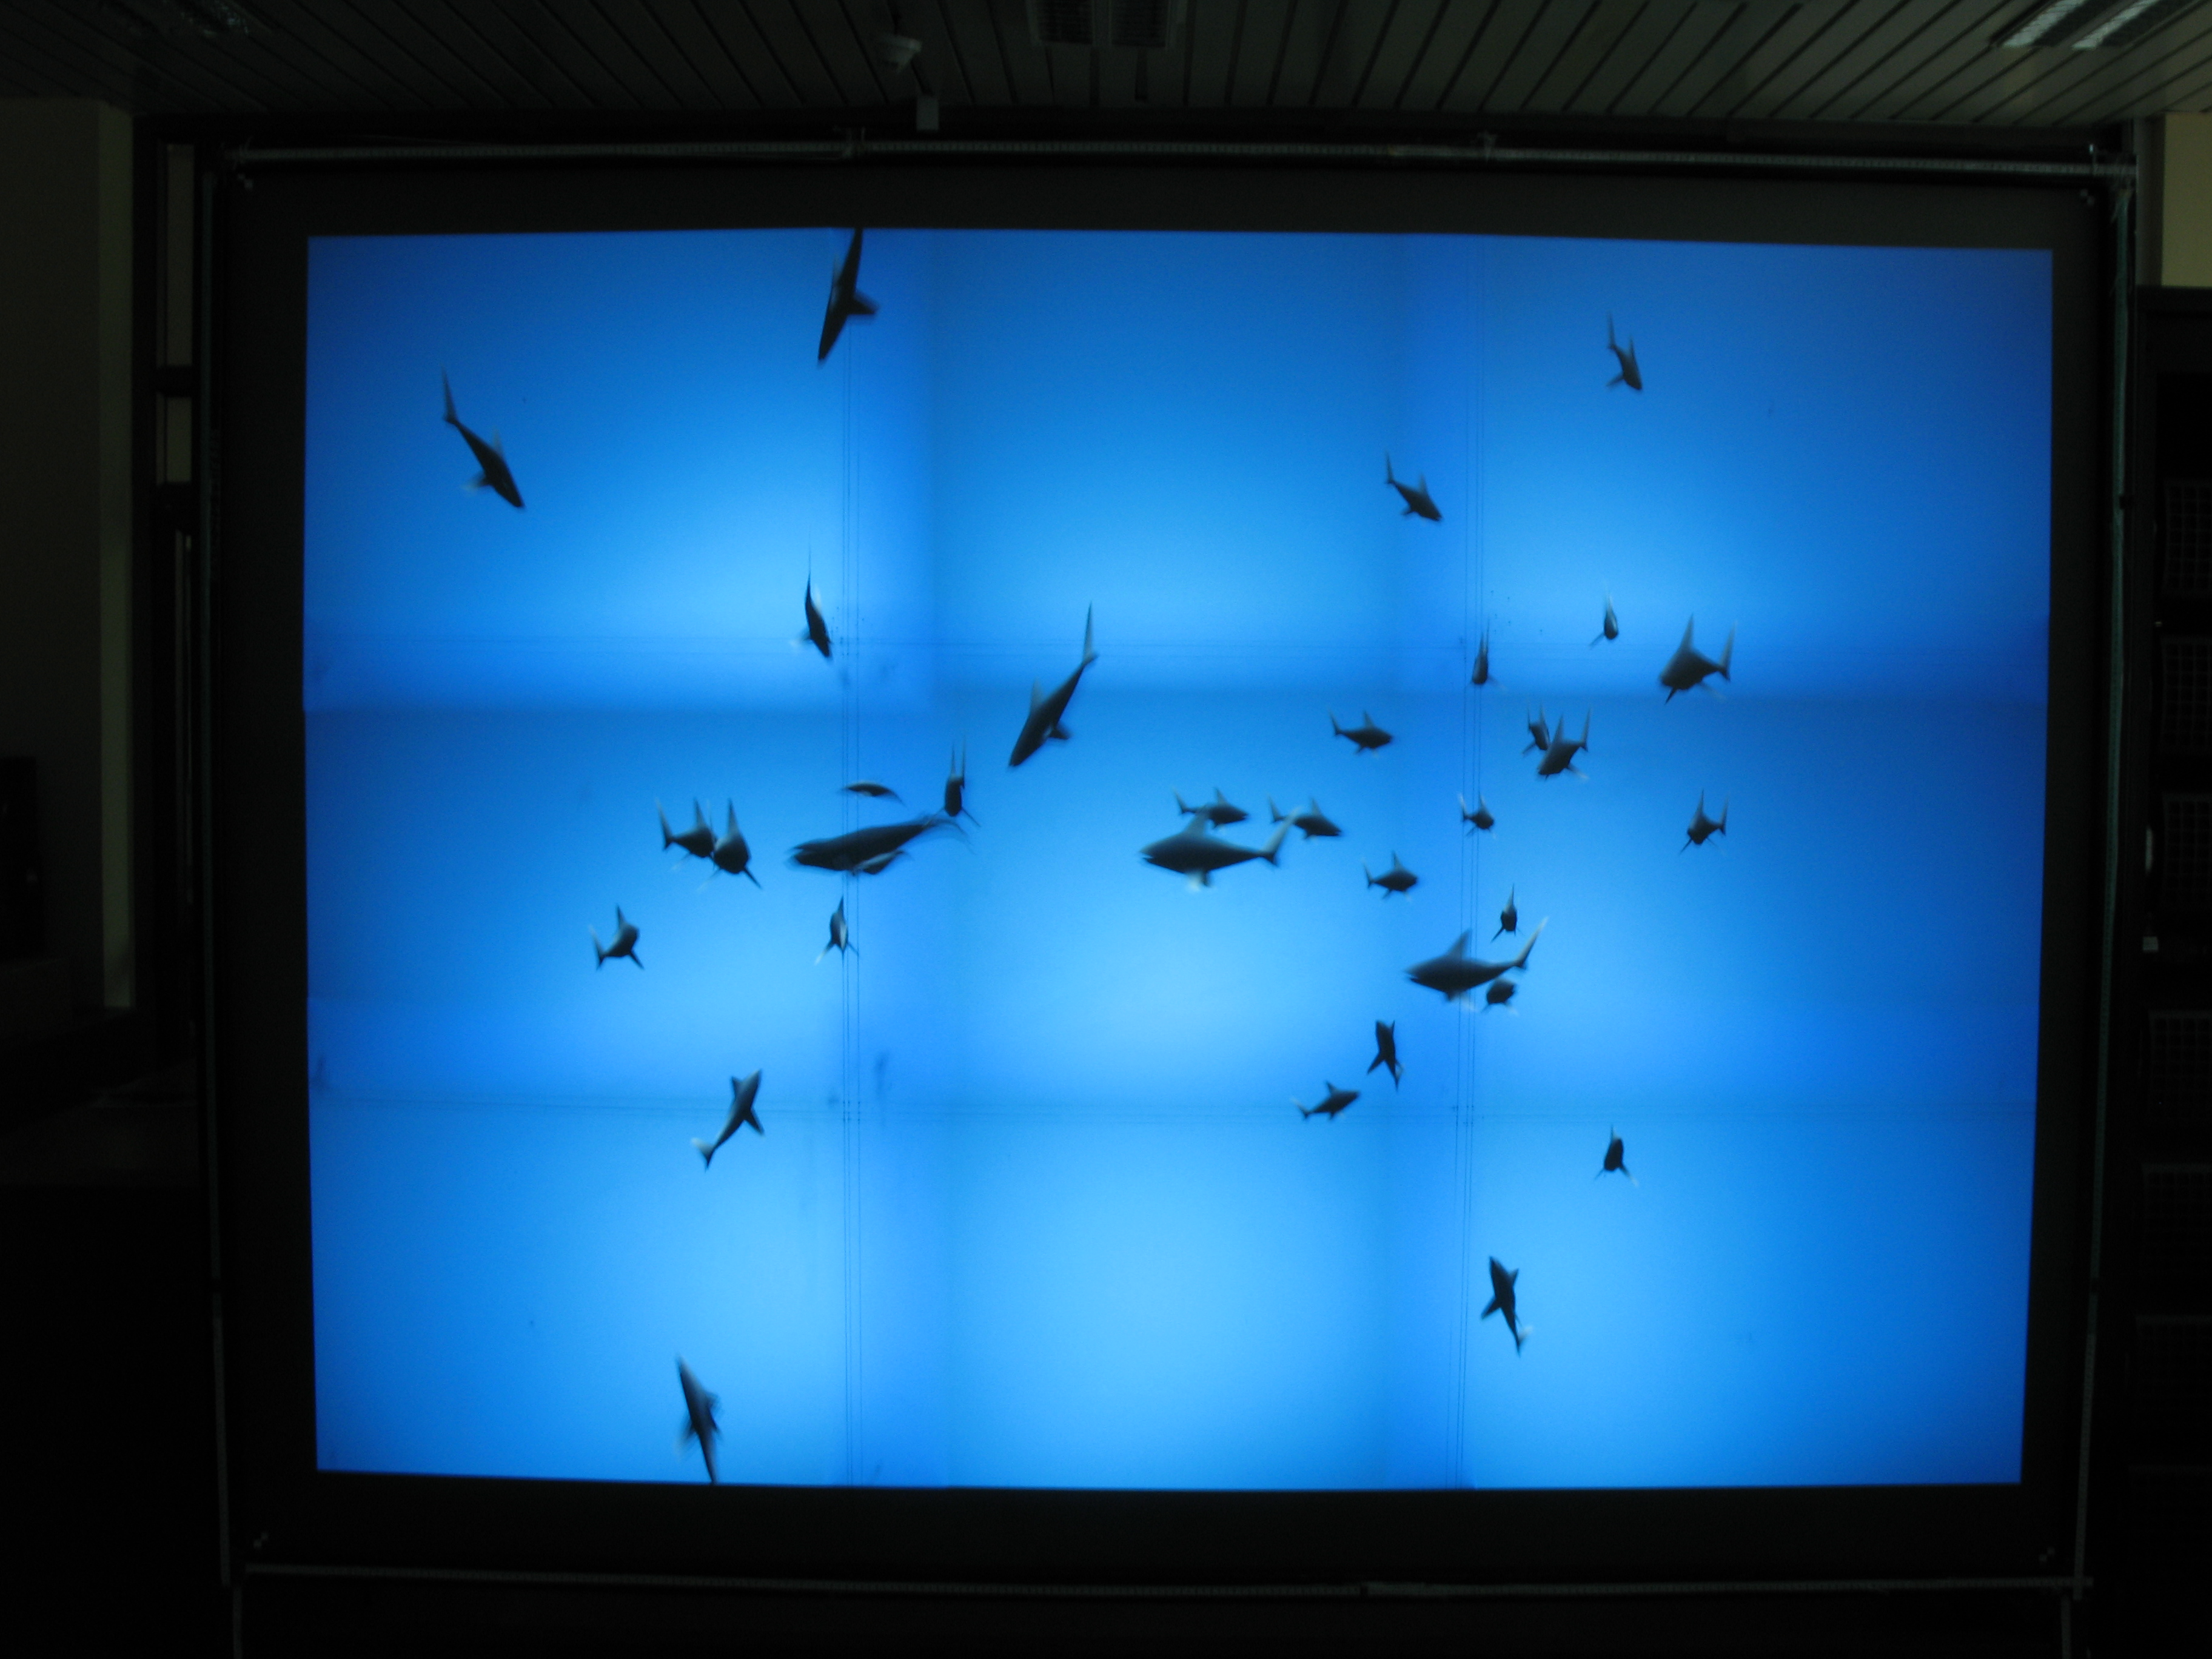
\includegraphics[width=11cm,height=8cm]{figures/with_cross_rat.jpg}
\caption{With cross ratio}
\label{cross_rat}
\end{figure}

\subsubsection{Geometric alignment accuracy}
Maximum misalignment on screen was found to be about 2.5mm across all inter-projector boundaries. A grid was projected across the display, figure \ref{misalign} shows the magnified view of maximum inter-projector misalignment observed after geometric registration.

\begin{figure}
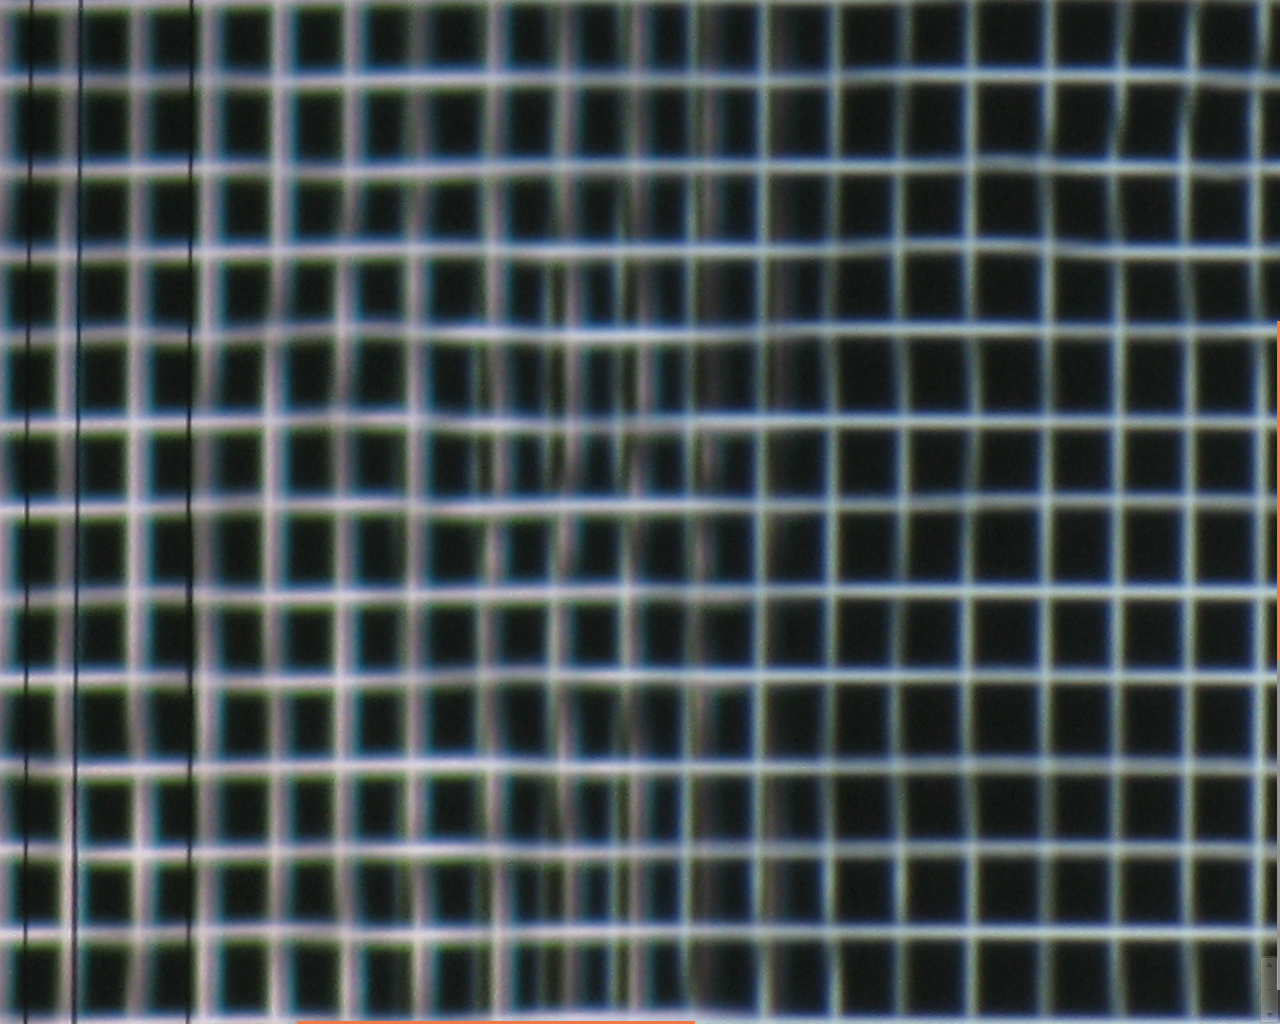
\includegraphics[width=11cm,height=8cm]{figures/misalign_1.png}
\caption{Magnified view of observed \textit{maximum} inter-projector misalignment}
\label{misalign}
\end{figure}



\section{Running the software}
In this section, we describe the steps to be followed to successfully run the developed software for geometric calibration and edge blending.
\subsection{Geometric calibration}

\subsection{Edge blending}



    

\section{Conclusions}
    We proposed and demonstrated \textit{Cross ratio} invariance based projection region recovery in Multiprojector geometric alignment problem. Brown's method puts constraint and limitation in which atleast outer features of neighboring projector must overlap in order to get geometrically continuous image on the screen. This actually limits their claimed merit of casual alignment of projector. Further, there was no provision for using projection region beyond outermost features. Cross ratio approach allows for recovery of artificial feature points at the endpoints of a projection region due to which full projection region can be utilized and there is no constraint on projector positioning.


\section{Future directions}
    Although inter-projector color seamlessness was attempted in this work through edge blending, perception of seamlessness is highly view-dependent. It was observed that applied blending works only at a particular viewpoint, changing viewpoint highlights the edges of neighboring projectors. In addition, luminance and chromaticity non-uniformities were observed not only across projectors but also within a projector's projection region. This issue has not been addressed by this work. Therefore, further work is required to attain inter and intra view independent color seamlessness in such systems. Solution to this problem will complete the main target of achieving seamless high resolution display where we cannot count number of projectors used behind the screen from any viewpoint. Work in this direction has been initiated with success for single view color seamlessness in \cite{2},\cite{3}. However, view independent color seamlessness still remains an open challenge. Scalability of system requires using multiple cameras in case complete screen cannot be captured by single camera. In such case, approach needs to be enhanced for registering feedback from multiple cameras to common coordinate system. Further extensions of the system includes adding support for non-planar screens.

\section{Acknowledgements}
    Author would like to thank Computer Graphics and Visualization section, Computer Division, BARC, Mumbai for providing valuable time, suggestions and infrastructure for this work.

\begin{thebibliography}{1}
\bibitem{1} 
Brown, M.S.; Seales, W.B., ``A practical and flexible tiled display system,'' Computer Graphics and Applications, 2002. Proceedings. 10th Pacific Conference on , vol., no., pp.194,203, 2002
doi: 10.1109/PCCGA.2002.1167859

\bibitem{2} 
Brown, M.; Majumder, A.; Ruigang Yang, ``Camera-based calibration techniques for seamless multiprojector displays,'' Visualization and Computer Graphics, IEEE Transactions on , vol.11, no.2, pp.193,206, March-April 2005
doi: 10.1109/TVCG.2005.27

\bibitem{3} 
Sajadi, B.; Lazarov, M.; Gopi, M.; Majumder, A., ``Color Seamlessness in Multi-Projector Displays Using Constrained Gamut Morphing,'' Visualization and Computer Graphics, IEEE Transactions on , vol.15, no.6, pp.1317,1326, Nov.-Dec. 2009
doi: 10.1109/TVCG.2009.124

\bibitem{4}
Greg Humphreys, Mike Houston, Ren Ng, Randall Frank, Sean Ahern, Peter D. Kirchner, and James T. Klosowski. 2002. Chromium: a stream-processing framework for interactive rendering on clusters. ACM Trans. Graph. 21, 3 (July 2002), 693-702. DOI=10.1145/566654.566639 http://doi.acm.org/10.1145/566654.566639

\bibitem{5}
Weblink:\newline
\url{en.wikipedia.org/wiki/Homography_(computer_vision)‎}

\end{thebibliography}



\end{document}
